\section{HexGame et stratégie gagnante}

Au Hex, pour toutes les tailles de plateaux, il existe une stratégie gagnante théorique pour le joueur qui commence.
Celle-ci n'est pas connue pour la plupart des tailles de plateaux, en effet elle demande une connaissance totale de toutes  
les parties possible ce qui n'est pas calculable en temps réaliste.

\paragraph{Stratégies gagnantes et arbre du jeu}
Modélisons le jeu de Hex à l'aide d'un arbre représentant toutes les parties possibles. L'arbre commence avec la position 
initiale, un plateau vide. De cette racine partent autant de branches qu'il y a de premiers coups. Ainsi, pour un plateau de
taille $2\times2$, on va retrouver 3 nœuds fils. Nous réitérons l'action à partir de chaque nœuds fils en leur rajoutant des branches vers
de nouveaux nœuds correspondant aux autres coups disponibles. Pour le plateau précédent; chaque fils possède alors 2 nouveaux fils.
\begin{figure}[h]
    \begin{center}
        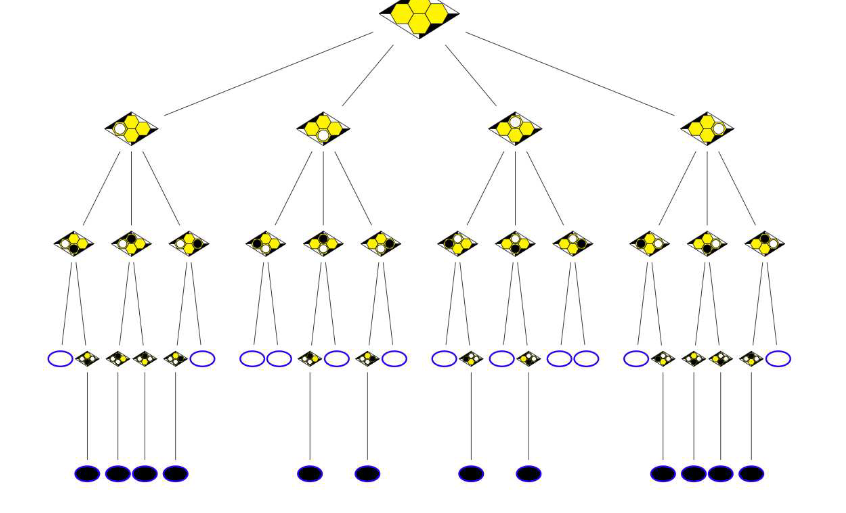
\includegraphics[width=0.4\textwidth]{root/strategie_gagnante.png}
    \end{center}
    \caption{Arbre complet pour un plateau $2\times2$}\label{fig:strategie_gagnante}
\end{figure}


L'arbre va nous aider à nous convaincre qu'il y a bien une stratégie gagnante pour l'un des deux joueurs. 
Le principe consiste à colorier tous les nœuds de l'arbre en blanc ou en noir. Chaque
nœud colorié correspond à une position à partir de laquelle le joueur de la couleur correspondante
possède une stratégie gagnante. 
Nous commençons par colorier en blanc (respectivement en noir) les feuilles représentant une victoire par les blancs
(respectivement par les noirs).
Nous souhaitons maintenant attribuer une couleur à un nœud qui n'en a pas encore. On remarque dans un premier temps que toutes les 
branches descendantes mènent à des nœuds déjà coloriés. Supposons que ce nœud représente une position où c'est 
aux blancs de jouer. Si au moins l'une des branches issues du nœud mène à un nœud blanc, alors on colorie le nœud
en blanc. Sinon, si toutes les branches mènent à des nœuds noirs, on le colorie en noir. On procède de la même façon si c'est 
aux noirs de jouer. De cette manière, nous sommes assurés de remplir l'arbre en entier de couleurs. La racine se voit donc attribuer 
une couleur. Ainsi, le premier joueur possède une stratégie gagnante.


\paragraph {Remarque:}
Pour un plateau de dimension $2\times2$, l'arbre possède un total de 24 feuilles et 52 branches.
il est calculé que pour le Hex a 11*11 la Game-tree complexity ou le nombre de feuilles de l'arbre est
approximativement 10^98 et le nombre de positions totales que peut prendre le jeu est de 2.4*10^56 contre
4.2*10^56
